\chapter{Results\label{cha:results}}

\ifdraft{In this section you discuss any issues that came up while developing
the system.  If you found something particularly interesting,
difficult, or an important learning experience, put it here.  This is
also a good place to put additional figures and data.}{}

The result section deals with presenting the different metrics discussed so far, within the RECAT-EU scheme. The data subset for the analysis was limited to four pair categories from the ICAO scheme: H-H, H-M, M-H, M-M. This simplification was done in order to filter out the insufficient data points from the other pairs for any valid conclusions.

\section{Inter-arrival Distance Separation of RECAT pairs}\label{sec:interarrival_dist_sep_RECAT}
The arrival pairs from the peak hour traffic at BIKF after re-categorisation are presented in Table~\ref{tab:pairs_mix_to_recat}. As expected from the traffic fleet analysis in \ref{ssec:traffic_mix}, most of the aircraft combined into C-C pairs. 

% Please add the following required packages to your document preamble:
% \usepackage{multirow}
% \usepackage{graphicx}
% \usepackage[table,xcdraw]{xcolor}
% If you use beamer only pass "xcolor=table" option, i.e. \documentclass[xcolor=table]{beamer}
\begin{table}[h]
\centering
\resizebox{\textwidth}{!}{%
\begin{tabular}{cc|c|c|c|c|c|c|}
\cline{3-8}
\multicolumn{1}{l}{} & \multicolumn{1}{l|}{} & \multicolumn{6}{c|}{Follower} \\ \cline{3-8} 
\multicolumn{1}{l}{} & \multicolumn{1}{l|}{} & CAT-A & CAT-B & CAT-C & CAT-D & CAT-E & CAT-F \\ \hline
\multicolumn{1}{|c|}{} & CAT-A &  &  &  & \cellcolor[HTML]{FFFFC7}1 &  &  \\ \cline{2-8} 
\multicolumn{1}{|c|}{} & CAT-B &  & \cellcolor[HTML]{FFFFC7}1 & \cellcolor[HTML]{FFFC9E}17 & \cellcolor[HTML]{FFFC9E}16 & \cellcolor[HTML]{FFFFC7}2 &  \\ \cline{2-8} 
\multicolumn{1}{|c|}{} & CAT-C &  & \cellcolor[HTML]{FFFC9E}19 & \cellcolor[HTML]{FD6864}1697 & \cellcolor[HTML]{FE996B}242 & \cellcolor[HTML]{FFCE93}41 & \cellcolor[HTML]{FFFC9E}14 \\ \cline{2-8} 
\multicolumn{1}{|c|}{} & CAT-D & \cellcolor[HTML]{FFFFC7}1 & \cellcolor[HTML]{FFFC9E}10 & \cellcolor[HTML]{FE996B}229 & \cellcolor[HTML]{FE996B}200 & \cellcolor[HTML]{FFFC9E}10 & \cellcolor[HTML]{FFFFC7}5 \\ \cline{2-8} 
\multicolumn{1}{|c|}{} & CAT-E &  & \cellcolor[HTML]{FFFFC7}1 & \cellcolor[HTML]{FFCE93}44 & \cellcolor[HTML]{FFFFC7}10 &  &  \\ \cline{2-8} 
\multicolumn{1}{|c|}{\multirow{-6}{*}{\rotatebox[origin=c]{90}{Leader}}} & CAT-F &  &  & \cellcolor[HTML]{FFFC9E}16 & \cellcolor[HTML]{FFFFC7}10 & \cellcolor[HTML]{FFFFC7}1 &  \\ \hline
\end{tabular}%
}
\caption[BIKF traffic mix sorted into RECAT-EU categories]{Number of RECAT pairs from the traffic mix at BIKF arranged into the corresponding wake categories. The majority of arrival pairs are classified as C-C.}
\label{tab:pairs_mix_to_recat}
\end{table}






\begin{figure}
    \centering
    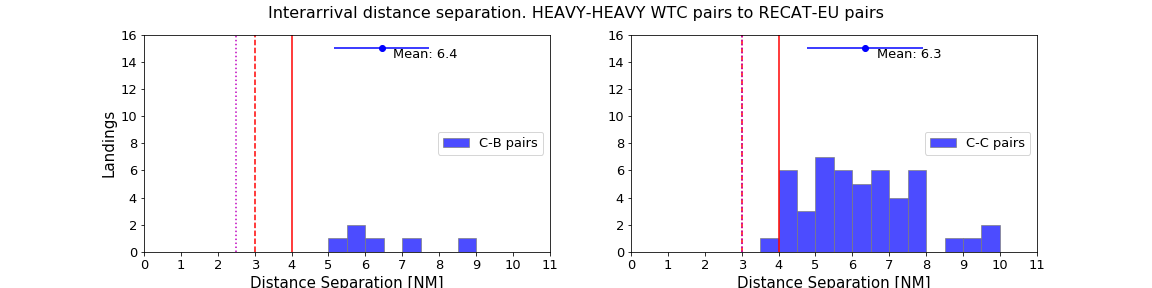
\includegraphics[width=1\textwidth]{graphics/fig_HH_to_RECAT_pairs_dist_separ.png}
    \caption[list of figures caption]{Caption}
    \label{fig:HH_to_RECAT_pairs_dist_separ}
\end{figure}

\begin{figure}
    \centering
    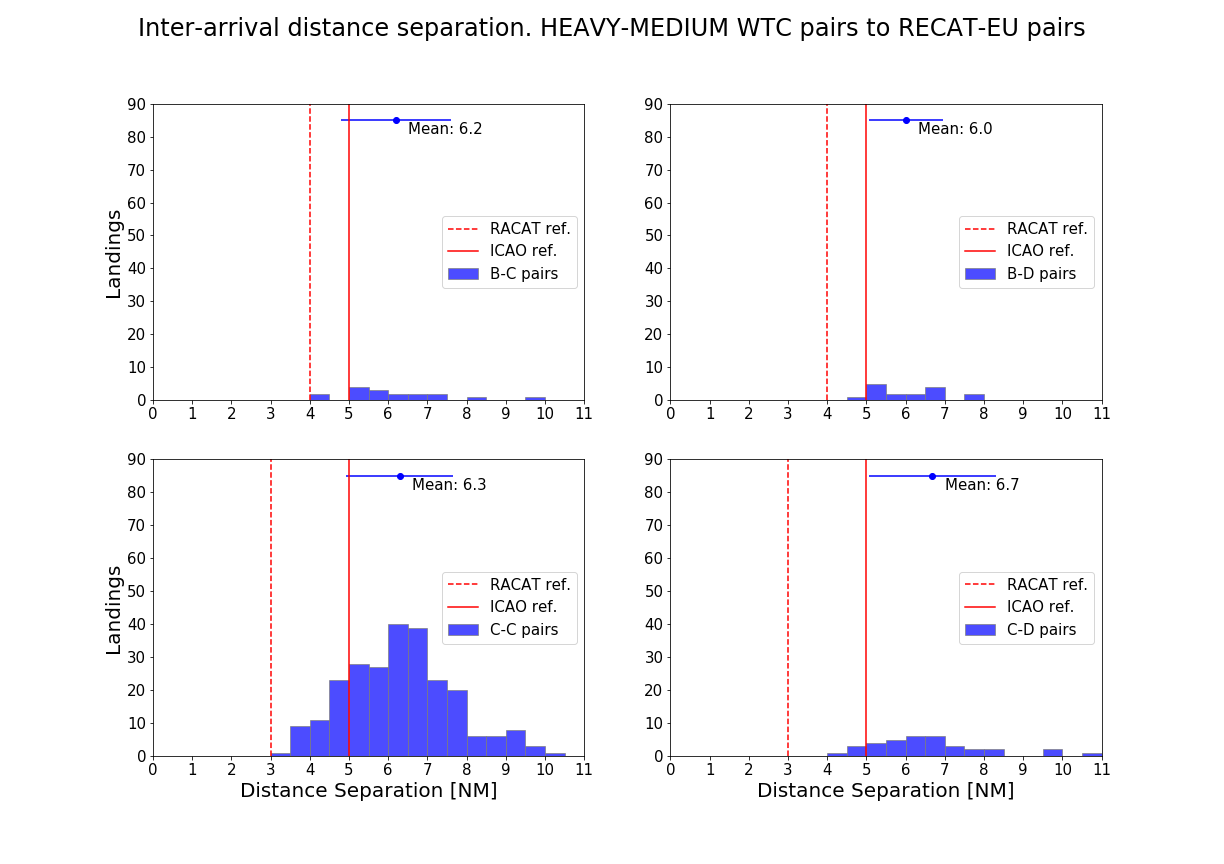
\includegraphics[width=1\textwidth]{graphics/fig_HM_to_RECAT_pairs_dist_separ.png}
    \caption[list of figures caption]{Caption}
    \label{fig:HM_to_RECAT_pairs_dist_separ}
\end{figure}

\begin{figure}
    \centering
    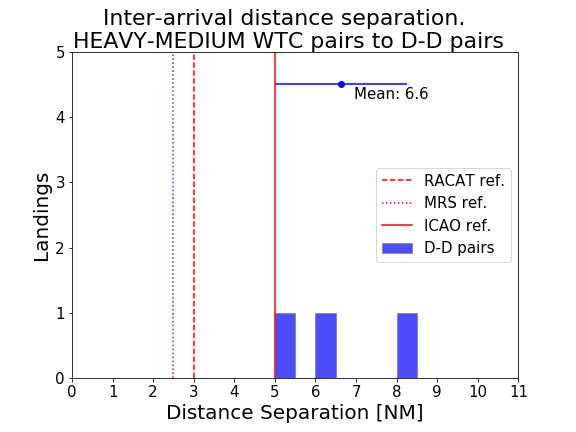
\includegraphics[width=0.5\textwidth]{graphics/fig_HM_to_DD_pairs_dist_separ.png}
    \caption[list of figures caption]{Caption}
    \label{fig:HM_to_DD_pairs_dist_separ}
\end{figure}



\begin{figure}[h]
    \centering
    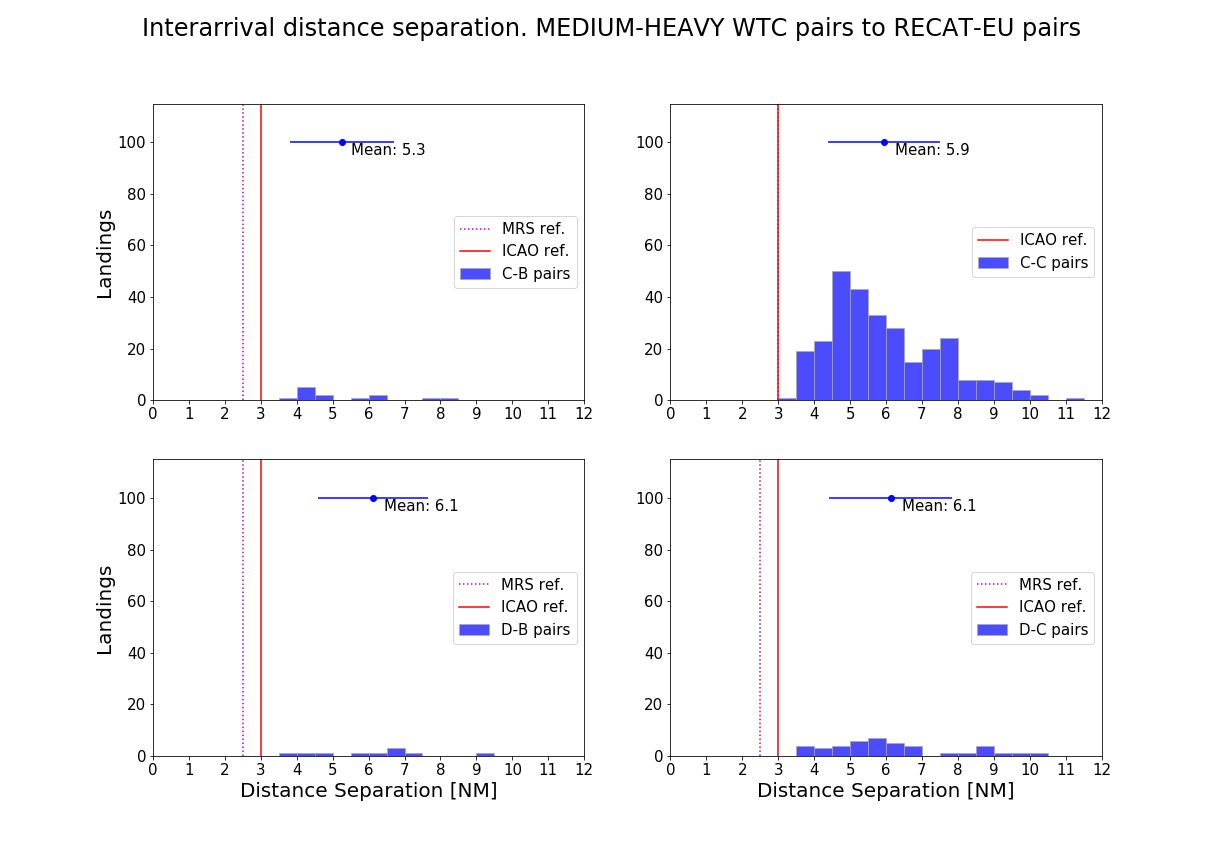
\includegraphics[width=1\textwidth]{graphics/fig_MH_to_RECAT_pairs_dist_separ.png}
    \caption[list of figures caption]{Caption}
    \label{fig:MH_to_RECAT_pairs_dist_separ}
\end{figure}

\begin{figure}[h]
    \centering
    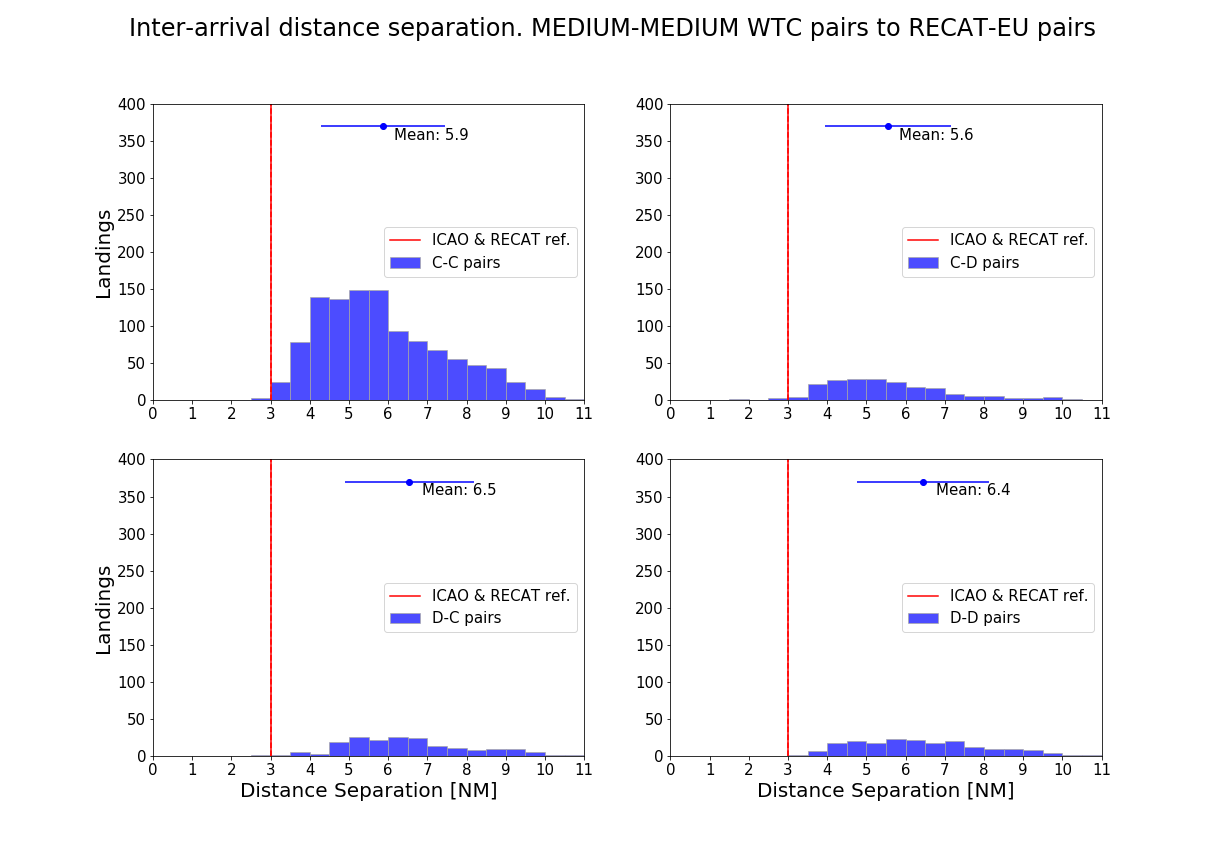
\includegraphics[width=1.0\textwidth]{graphics/fig_MM_to_RECAT_pairs_dist_separ.png}
    \caption[list of figures caption]{Caption}
    \label{fig:MM_to_RECAT_pairs_dist_separ}
\end{figure}

\begin{figure}[h]
    \centering
    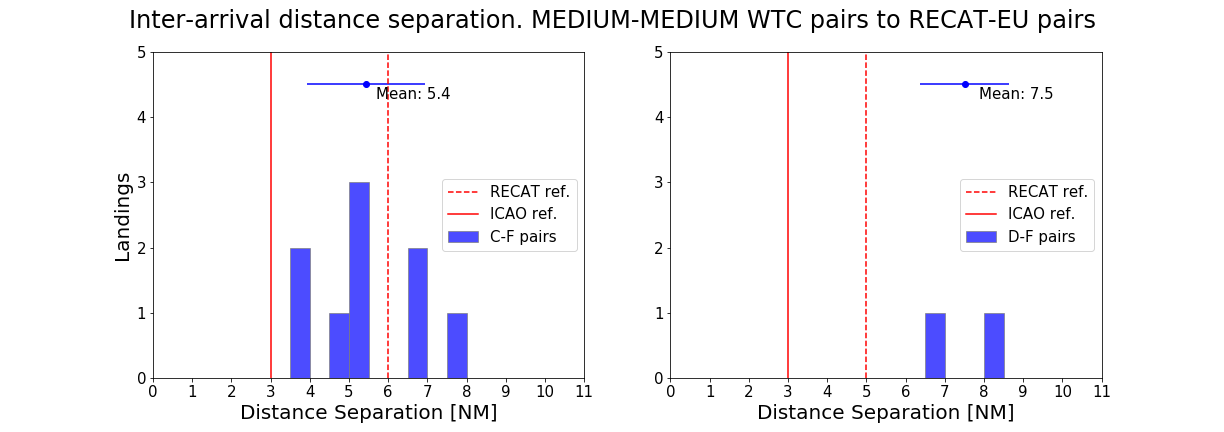
\includegraphics[width=1\textwidth]{graphics/fig_MM_to_CF_and_DF_pairs_dist_separ.png}
    \caption[list of figures caption]{Caption}
    \label{fig:MM_to_CF_and_DF_pairs_dist_separ}
\end{figure}


\section{Runway Occupancy and Landing Time Interval for RECAT pairs}




\begin{figure}[h]
    \centering
    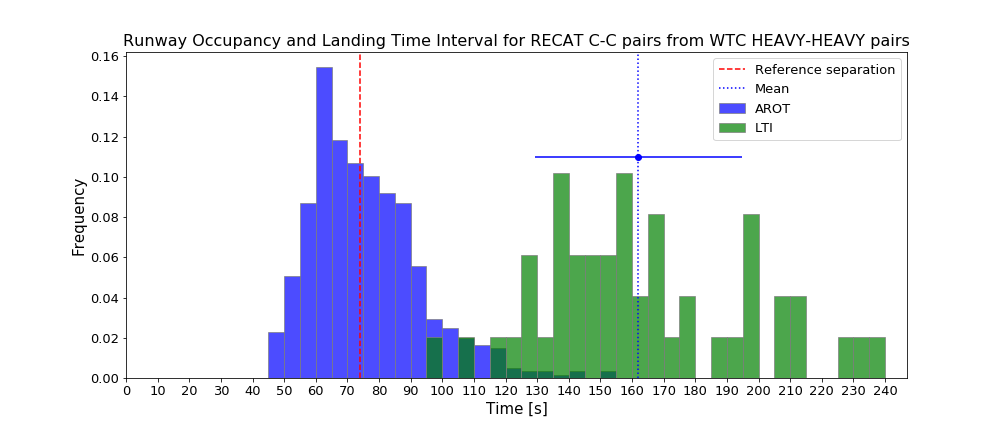
\includegraphics[width=1\textwidth]{graphics/fig_CC_from_HH_pairs_time_sep.png}
    \caption[list of figures caption]{Caption}
    \label{fig:CC_from_HH_pairs_time_sep}
\end{figure}




\begin{figure}[h]
    \centering
    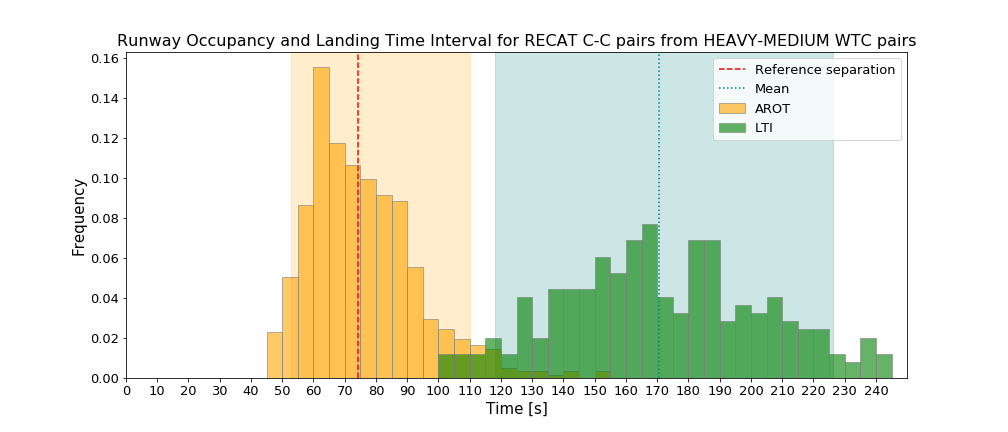
\includegraphics[width=1\textwidth]{graphics/fig_CC_from_HM_pairs_time_sep.png}
    \caption[list of figures caption]{Caption}
    \label{fig:CC_from_HM_pairs_time_sep}
\end{figure}

\begin{figure}[h]
    \centering
    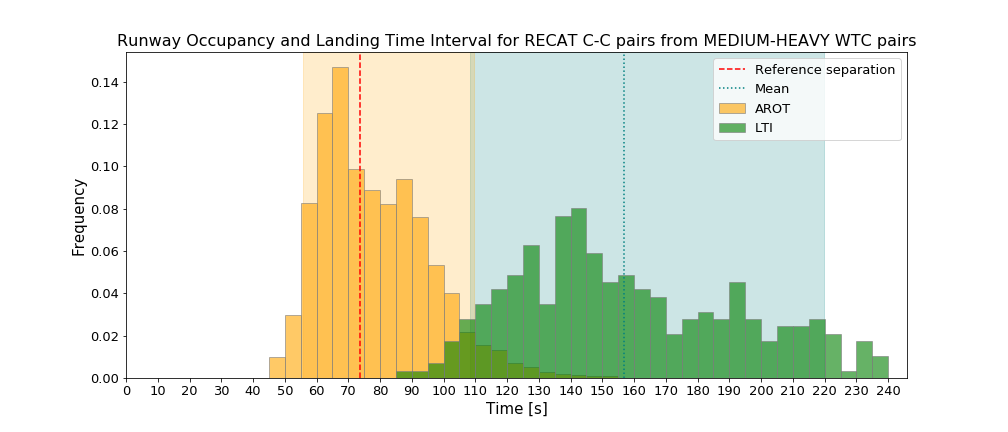
\includegraphics[width=1\textwidth]{graphics/fig_CC_from_MH_pairs_time_sep.png}
    \caption[list of figures caption]{Caption}
    \label{fig:CC_from_MH_pairs_time_sep}
\end{figure}

\begin{figure}[h]
    \centering
    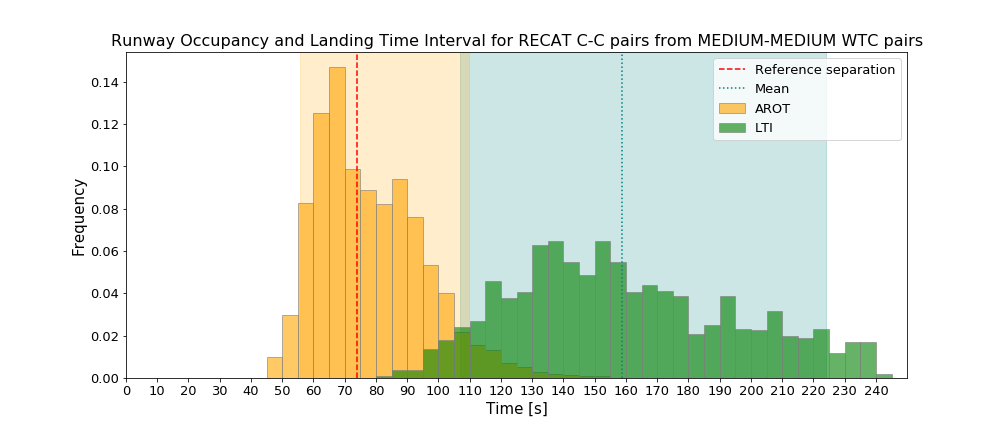
\includegraphics[width=1\textwidth]{graphics/fig_CC_from_MM_pairs_time_sep.png}
    \caption[list of figures caption]{Caption}
    \label{fig:CC_from_MM_pairs_time_sep}
\end{figure}

\begin{figure}[h]
    \centering
    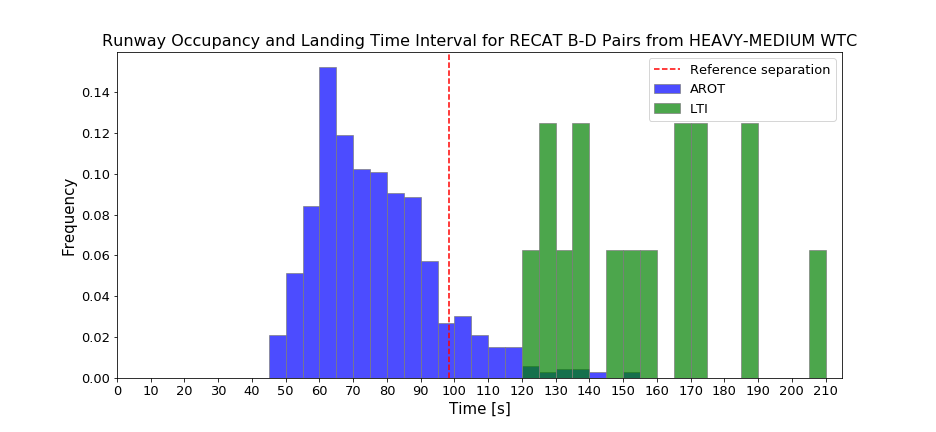
\includegraphics[width=1\textwidth]{graphics/fig_BD_from_HM_pairs_time_sep.png}
    \caption[list of figures caption]{Caption}
    \label{fig:BD_from_HM_pairs_time_sep}
\end{figure}







% \lipsum[28-34]

%%% Local Variables: 
%%% mode: latex
%%% TeX-master: "DEGREE-NAME-YEAR"
%%% End: 
